%%%%%%%%%%%%%%%%%%%%%%%%%%%%%%%%%%%%%%%%%
% This template is created by Zhou Feng on 2/21/2019 for the undergraduate thesis
%opening speech at Huazhong University of Science and Technlogy

%----------------------------------------------------------------------------------------
%	PACKAGES AND THEMES
%----------------------------------------------------------------------------------------

\documentclass{beamer}

%----------------------------------------------------------------%
%% For Math Symbols, 载入常用的数学包, 符号包
\usepackage{amsmath}
\usepackage{amsfonts}
\usepackage{amssymb}
\usepackage{mathrsfs}

%----------------------------------------------------------------%
%% For the fonts (style, color, size).字体的大小,颜色,以及定义常用的字号
\usepackage{ctex}% If you are lazy, the CTEX suit is enough.
% Chinese Font
\usepackage{xeCJK}% For the Chinese through XeLaTex
\setCJKmainfont{SimSun} % set the mainfont of Chinese as songti. (serif) for  
\setCJKsansfont{SimSun} % sans serif font for \textsf
\setCJKmonofont{SimSun} % monospace font for \texttt
% \punctstyle{kaiming}   % Remove the space used by symbols like comma. Special for the mainland students like us HUSTers.
\setCJKfamilyfont{song}{SimSun}                             %宋体 song
\newcommand{\song}{\CJKfamily{song}}                        
\setCJKfamilyfont{kai}{KaiTi_GB2312}                        %楷体2312  kai
\newcommand{\kai}{\CJKfamily{kai}}  
\setCJKfamilyfont{hwzs}{STZhongsong}                        %华文中宋  hwzs
\newcommand{\hwzs}{\CJKfamily{hwzs}}
% English Font
\usepackage{fontspec}% Then you can use the fonts installed at your device. 
\setmainfont{Times New Roman}
\setsansfont{Times New Roman}
\setmonofont{Times New Roman}
%\setsansfont{[foo.ttf]} % for the fonts at this default path.
% Font Color 利用definecolor自己可以定义颜色
\usepackage{xcolor}
\definecolor{MSBlue}{rgb}{.204,.353,.541}
\definecolor{MSLightBlue}{rgb}{.31,.506,.741}
% Font Size (I use pinyin represents the corresponding size in Microsorft Word)
% \newcommand{\chuhao}{\fontsize{42pt}{\baselineskip}\selectfont}
% \newcommand{\xiaochuhao}{\fontsize{36pt}{\baselineskip}\selectfont}
% \newcommand{\yihao}{\fontsize{28pt}{\baselineskip}\selectfont}
% \newcommand{\erhao}{\fontsize{21pt}{\baselineskip}\selectfont}
% \newcommand{\xiaoerhao}{\fontsize{18pt}{\baselineskip}\selectfont}
% \newcommand{\sanhao}{\fontsize{15.75pt}{\baselineskip}\selectfont}
\newcommand{\sihao}{\fontsize{14pt}{18pt}\selectfont}
\newcommand{\xiaosihao}{\fontsize{12pt}{18pt}\selectfont}
\newcommand{\wuhao}{\fontsize{10.5pt}{18pt}\selectfont}
% \newcommand{\xiaowuhao}{\fontsize{9pt}{\baselineskip}\selectfont}
% \newcommand{\liuhao}{\fontsize{7.875pt}{\baselineskip}\selectfont}
% \newcommand{\qihao}{\fontsize{5.25pt}{\baselineskip}\selectfont}

% 还可以输出伪斜体
%{\CJKfontspec[FakeSlant = 0.2]{STSong}伪斜体(华文宋体)}


%----------------------------------------------------------------%
%% For the caption and reference 图表及公式的编号规范
\usepackage{caption}
\captionsetup[figure]{labelformat=default, labelsep=quad,name={图}}
\captionsetup[table]{labelformat=default,labelsep=quad,name={表}}
%设置图表标题的计数方式
\renewcommand{\thefigure}{\thesection--\arabic{figure}} % set caption label style to 2-1 
\renewcommand{\thetable}{\thesection--\arabic{table}} % set caption label style to 2-1 
\captionsetup[figure]{labelfont=normalfont,textfont=normalfont} 
\captionsetup[table]{labelfont=normalfont,textfont=normalfont} 
%设置图表的autoref的格式
\newcommand{\reffig}[1]{图 \ref{#1}}
\newcommand{\reftab}[1]{表 \ref{#1}}
\newcommand{\refeq}[1]{公式 \ref{#1}}
\newcommand{\refprop}[1]{命题 \ref{#1}}
\newcommand{\reflmm}[1]{引理 \ref{#1}}
%公式的编号格式
\numberwithin{equation}{section}
\renewcommand\theequation{\arabic{section}--\arabic{equation}}
%----------------------------------------------------------------%
%% 设置幻灯片的格式 set the theme, colorstyle, and other options for this beamer slides. I have included many alternative options for you. As a student from HUST, I prefer the default Madrid theme.
\mode<presentation> {

% The Beamer class comes with a number of default slide themes
% which change the colors and layouts of slides. Below this is a list
% of all the themes, uncomment each in turn to see what they look like.

%\usetheme{default}
%\usetheme{AnnArbor}
%\usetheme{Antibes}
%\usetheme{Bergen}
%\usetheme{Berkeley}
%\usetheme{Berlin}
%\usetheme{Boadilla}
%\usetheme{CambridgeUS}
%\usetheme{Copenhagen}
%\usetheme{Darmstadt}
%\usetheme{Dresden}
%\usetheme{Frankfurt}
%\usetheme{Goettingen}
%\usetheme{Hannover}
%\usetheme{Ilmenau}
%\usetheme{JuanLesPins}
%\usetheme{Luebeck}
\usetheme{Madrid}
%\usetheme{Malmoe}
%\usetheme{Marburg}
%\usetheme{Montpellier}
%\usetheme{PaloAlto}
%\usetheme{Pittsburgh}
%\usetheme{Rochester}
%\usetheme{Singapore}
%\usetheme{Szeged}
%\usetheme{Warsaw}

% As well as themes, the Beamer class has a number of color themes
% for any slide theme. Uncomment each of these in turn to see how it
% changes the colors of your current slide theme.

%\usecolortheme{albatross}
%\usecolortheme{beaver}
%\usecolortheme{beetle}
%\usecolortheme{crane}
%\usecolortheme{dolphin}
%\usecolortheme{dove}
%\usecolortheme{fly}
%\usecolortheme{lily}
%\usecolortheme{orchid}
%\usecolortheme{rose}
%\usecolortheme{seagull}
%\usecolortheme{seahorse}
%\usecolortheme{whale}
%\usecolortheme{wolverine}

%\setbeamertemplate{footline} % To remove the footer line in all slides uncomment this line
%\setbeamertemplate{footline}[page number] % To replace the footer line in all slides with a simple slide count uncomment this line

%\setbeamertemplate{navigation symbols}{} % To remove the navigation symbols from the bottom of all slides uncomment this line
}





%----------------------------------------------------------------%
%% For the fonts (style, color, size).字体的大小,颜色,以及定义常用的字号
%\usepackage{ctex}% If you are lazy, the CTEX suit is enough.
% Chinese Font
\usepackage{xeCJK}% For the Chinese through XeLaTex
\setCJKmainfont{SimSun} % set the mainfont of Chinese as songti. (serif) for  
\setCJKsansfont{SimSun} % sans serif font for \textsf
\setCJKmonofont{SimSun} % monospace font for \texttt
\punctstyle{kaiming}   % Remove the space used by symbols like comma. Special for the mainland students like us HUSTers.
%\setCJKfamilyfont{song}{SimSun}                             %宋体 song
%\newcommand{\song}{\CJKfamily{song}}                        
%\setCJKfamilyfont{kai}{KaiTi_GB2312}                        %楷体2312  kai
%\newcommand{\kai}{\CJKfamily{kai}}  
%\setCJKfamilyfont{hwzs}{STZhongsong}                        %华文中宋  hwzs
%\newcommand{\hwzs}{\CJKfamily{hwzs}}
% English Font
\usepackage{fontspec}% Then you can use the fonts installed at your device. 
\setmainfont{Times New Roman}
\setsansfont{Times New Roman}
\setmonofont{Times New Roman}
%\setsansfont{[foo.ttf]} % for the fonts at this default path.
% Font Color 利用definecolor自己可以定义颜色
\usepackage{xcolor}
\definecolor{MSBlue}{rgb}{.204,.353,.541}
\definecolor{MSLightBlue}{rgb}{.31,.506,.741}
% Font Size (I use pinyin represents the corresponding size in Microsorft Word)
% \newcommand{\chuhao}{\fontsize{42pt}{\baselineskip}\selectfont}
% \newcommand{\xiaochuhao}{\fontsize{36pt}{\baselineskip}\selectfont}
% \newcommand{\yihao}{\fontsize{28pt}{\baselineskip}\selectfont}
% \newcommand{\erhao}{\fontsize{21pt}{\baselineskip}\selectfont}
% \newcommand{\xiaoerhao}{\fontsize{18pt}{\baselineskip}\selectfont}
% \newcommand{\sanhao}{\fontsize{15.75pt}{\baselineskip}\selectfont}
%\newcommand{\sihao}{\fontsize{14pt}{18pt}\selectfont}
%\newcommand{\xiaosihao}{\fontsize{12pt}{18pt}\selectfont}
%\newcommand{\wuhao}{\fontsize{10.5pt}{18pt}\selectfont}
% \newcommand{\xiaowuhao}{\fontsize{9pt}{\baselineskip}\selectfont}
% \newcommand{\liuhao}{\fontsize{7.875pt}{\baselineskip}\selectfont}
% \newcommand{\qihao}{\fontsize{5.25pt}{\baselineskip}\selectfont}

%----------------------------------------------------------------%
%% For the style of theorems, definitions, proofs and remarks 定义数学里面一些常用的环境
\usepackage{amsthm}
\newtheorem{thm}{\textbf{定理}}[section]
%The section in [] can be replaced by chapter or subsection
\theoremstyle{definition} \newtheorem{law}[thm]{Law}
\theoremstyle{plain} \newtheorem{jury}[thm]{Jury}
\theoremstyle{remark} \newtheorem*{marg}{Margaret}

\usepackage{graphicx} % Allows including images
\usepackage{booktabs} % Allows the use of \toprule, \midrule and \bottomrule in tables


%----------------------------------------------------------------%
%Something to improve my work efficiency.
\newcommand{\comma}{\text{,}}
\newcommand{\juhao}{\text{。}}
\newcommand{\fenhao}{\text{;}}
\newcommand{\pmone}{\pm1}
\newcommand{\xysolution}[2]{$ x=#1\comma y=#2 $}
\newcommand{\conalpha}{$ \alpha=\left[a_{1},a_{2},a_{3},\ldots\right] $}
\newcommand{\parquo}[1]{$ p_{#1}/q_{#1}=\left[a_{1},\ldots,a_{#1-1}\right] $}
\newcommand{\qfield}[1]{$ \mathbf{Q}\left(\sqrt{#1}\right) $}%二次域每次输入太麻烦了,
\newcommand{\pelleq}[2]{ $ x^{2}-#1y^{2}=#2 $} % Pell方程
\newcommand{\mymod}[3]{$ #1\equiv#2\left(\!\!\mod#3\right) $}
\newcommand{\periodrep}[3]{$ \sqrt{#1}=\left[#2;\overline{#3}\right] $}
\newcommand{\erfenzy}{\dfrac{1}{2}}
\newcommand{\mathmod}[3]{ #1\equiv#2\left(\!\!\mod#3\right) }
\newcommand{\mathnotmod}[3]{ #1\not\equiv#2\left(\!\!\mod#3\right) }
\newcommand{\dekd}{D\left(H,K\right)}
\newcommand{\dekdKH}{D\left(K,H\right)}
\newcommand{\ddek}[2]{D\left(H_{#1},H_{#2}\right)}
\newcommand{\gdek}[2]{g\left(H_{#1},H_{#2}\right)}
\newcommand{\myone}[1]{\left(-1\right)^{#1}} 

%----------------------------------------------------------------------------------------
%	TITLE PAGE 标题页
%----------------------------------------------------------------------------------------

\title[开题答辩]{Bernoulli卷积的性质 \\ \small{毕业设计开题答辩}} % The short title appears at the bottom of every slide, the full title is only on the title page

\author{冯洲} % Your name
\institute[HUST] % Your institution as it will appear on the bottom of every slide, may be shorthand to save space
{
华中科技大学 \\ % Your institution for the title page
\medskip
\textit{U201510104@hust.edu.cn} % Your email address
}
\date{\today} % Date, can be changed to a custom date

\begin{document}

\begin{frame}
\titlepage % Print the title page as the first slide
\end{frame}


\begin{frame}
\frametitle{目录} % Table of contents slide, comment this block out to remove it
\tableofcontents % Throughout your presentation, if you choose to use \section{} and \subsection{} commands, these will automatically be printed on this slide as an overview of your presentation
\end{frame}

%----------------------------------------------------------------------------------------
%	PRESENTATION SLIDES
%----------------------------------------------------------------------------------------

%------------------------------------------------
\section{选题背景} % Sections can be created in order to organize your presentation into discrete blocks, all sections and subsections are automatically printed in the table of contents as an overview of the talk
%------------------------------------------------

%\subsection{Subsection Example} % A subsection can be created just before a set of slides with a common theme to further break down your presentation into chunks

\begin{frame}
\frametitle{Bernoulli卷积简介}\small
Bernoulli卷积是一类简单而有趣的自相似测度。令$ \nu_{\lambda} $为随机级数$ \sum_{0}^{\infty} \pmone\lambda^{n} $分布,其中的符号以概率$ \frac{1}{2} $独立地取得。这正是测度$ \frac{1}{2}(\delta_{-\lambda^{n}}+\delta_{\lambda^{n}}) $的无穷卷积,因此叫``Bernoulli卷积''。关于这类测度的研究可以追溯到1930年,Bernoulli卷积与调和分析,代数数理论,动力系统,以及Hausdorff维数的估计等领域有紧密的联系。


根据不同的研究领域,Bernoulli卷积有不同的表示形式。\cite{Sixtyyears}

\end{frame}

\begin{frame}

\frametitle{Bernoulli卷积基本问题}\small
根据\cite{DJFeng1},对$ \beta\in(1,2) $,Bernoulli卷积$ \nu_{\beta} $可以定义为下面一族测度$ \nu_{\beta}^{n} $的weak-star极限
\[ \nu_{\beta}^{n}:= \dfrac{1}{2}\sum_{a_{1}\cdots a_{n}\in \lbrace0,1\rbrace}\delta_{\sum_{i=1}^{n}a_{i}\beta^{-i}}\quad\juhao \]

关于Bernoulli卷积基本问题是:对于哪些$ \beta $,这个测度是绝对连续的,哪些是奇异的(singular)。如果密度(关于Lebesgue测度的Radon-Nikodym导数)存在,那么它的光滑性如何($ L^{p?}$)? 然后就是Bernoulli
卷积的Hausdorff维数如何,是否等于1,怎样去估计Hausdorff维数。

其中有一个非常重要的结果就是,Erd\"os证明如果$ \beta $为Pisot数,那么相应的Bernoulli卷积的维数一定小于1。
\begin{block}{一个open的问题}
	如果$ \nu_{\beta} $奇异,那么是否一定有$ \beta $为Pisot数?
\end{block}
\end{frame}



%------------------------------------------------
%------------------------------------------------
\section{课题内容及拟采用方法} 
%------------------------------------------------

\begin{frame}
\frametitle{课题内容及拟采用方法}
\begin{columns}[c]
	\column{.45\textwidth}
	\small
根据需要,将Bernoulli卷积定义为:对于作用在$ \left[0,1\right] $上的IFS: $ S=\lbrace S_{1}=\frac{1}{\beta}x,S_{2}=\frac{1}{\beta}x+1-\frac{1}{\beta}\rbrace $,有下自相似测度
\[ \nu_{\beta}(A)=\erfenzy\nu_{\beta}\left(S_{1}^{-1}(A)\right)+\erfenzy\nu_{\beta}\left(S_{2}^{-1}(A)\right) \juhao\]

\column{.45\textwidth}
\begin{figure}
\centering
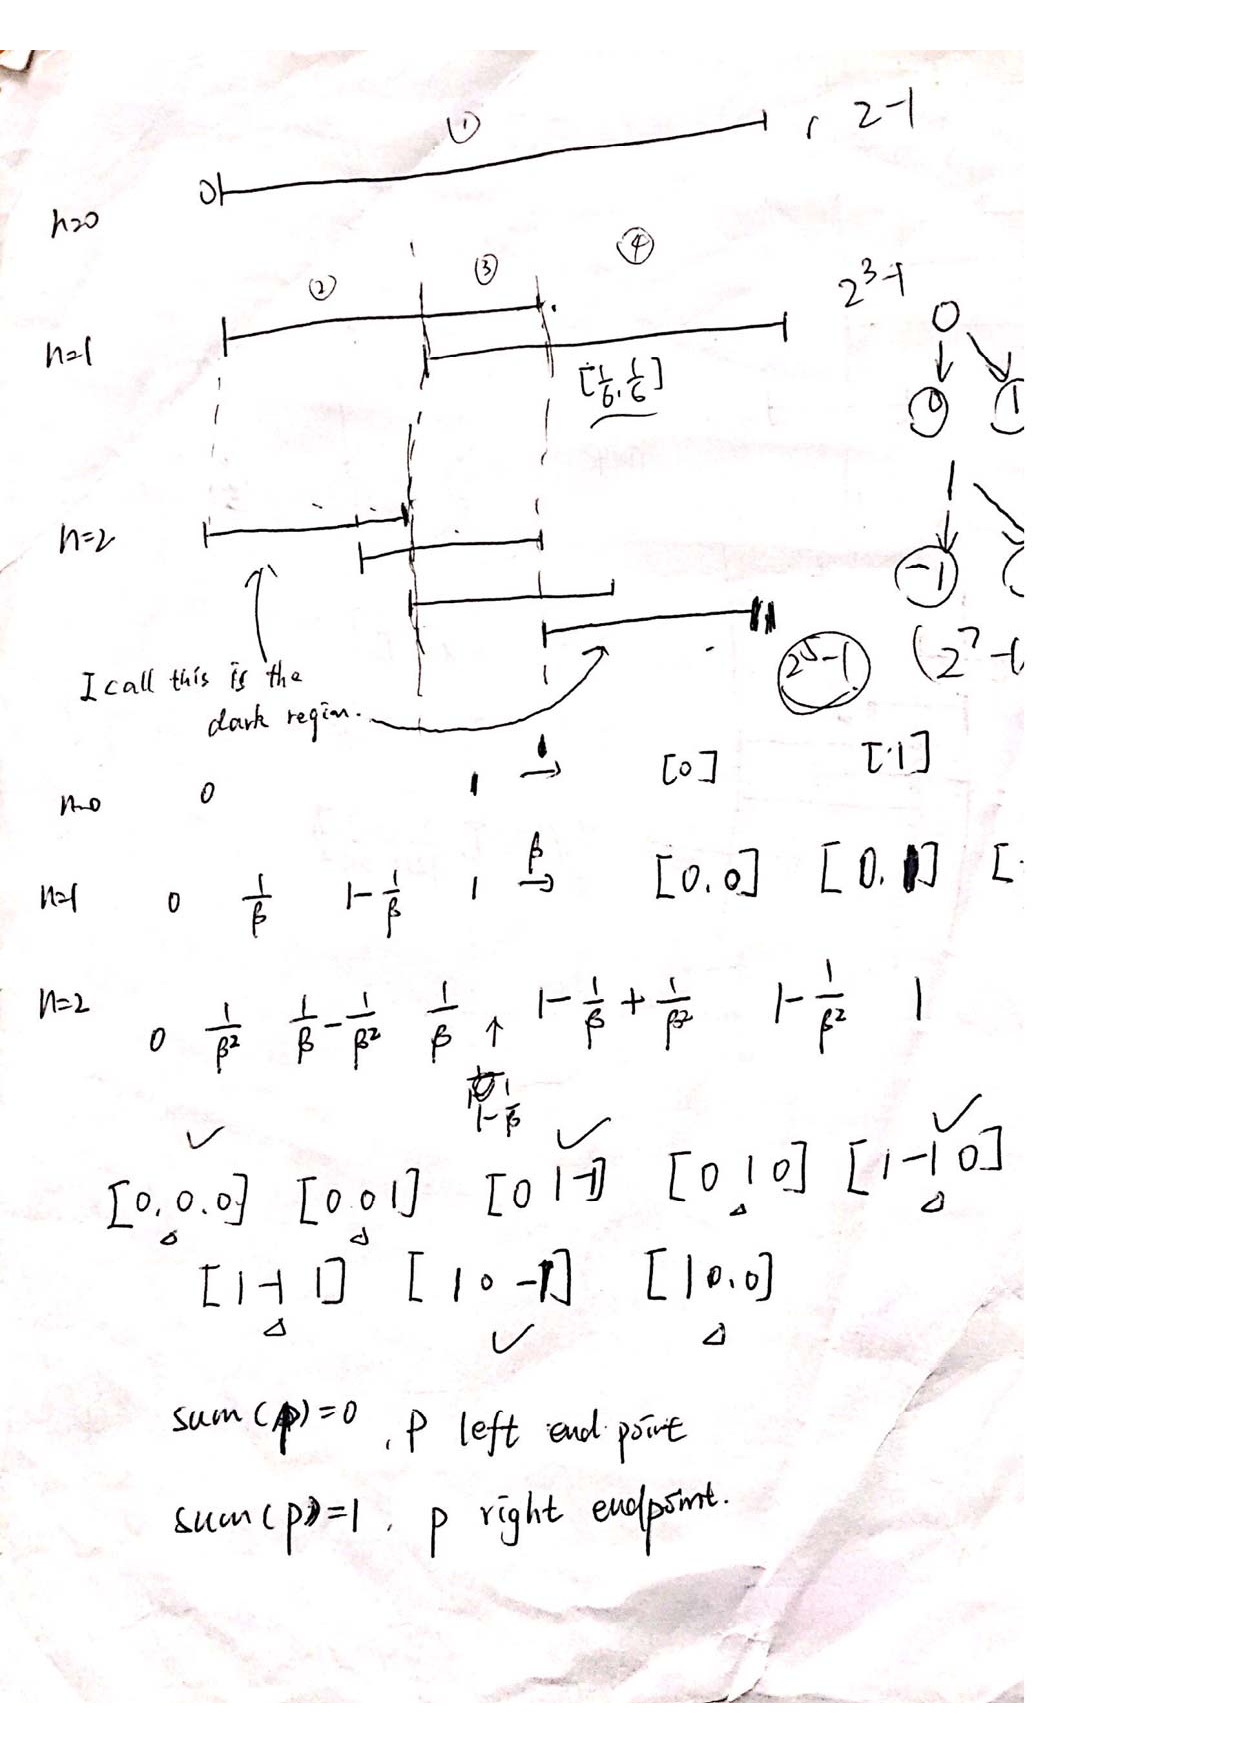
\includegraphics[width=0.6\linewidth,height=0.5\textheight]{system}
\caption{单位区间上的IFS}
\end{figure}
\end{columns}
\end{frame}




\begin{frame}
\frametitle{课题内容及拟采用方法}
\begin{itemize}
	\item 基于之前关于Bernoulli卷积的表示形式,阅读论文\cite{DJFeng1}\cite{DJFeng2}\cite{DJFeng3}\cite{Niki1},向指导老师需求帮助,利用Matlab实现其中的Hausdorff维数估计公式。对于满足算法条件的$ \beta $,实现算法估计相应的$ \nu_{\beta} $的Hausdoff维数。
	\item 阅读相关的课本,书籍及论文\cite{Falconer}\cite{Mattila},学习理解Bernoulli卷积的理论知识,进一步理解上面维数估计式之间的联系。争取对Bernoulli卷积的性质有一定的认识。
	\item 总结学习到的知识,整理实践结果,完成毕业论文的写作。
\end{itemize}
\end{frame}


%------------------------------------------------




%------------------------------------------------
\section{可能得到结果}
%------------------------------------------------
\begin{frame}
\frametitle{可能得到结果}
	\begin{figure}
		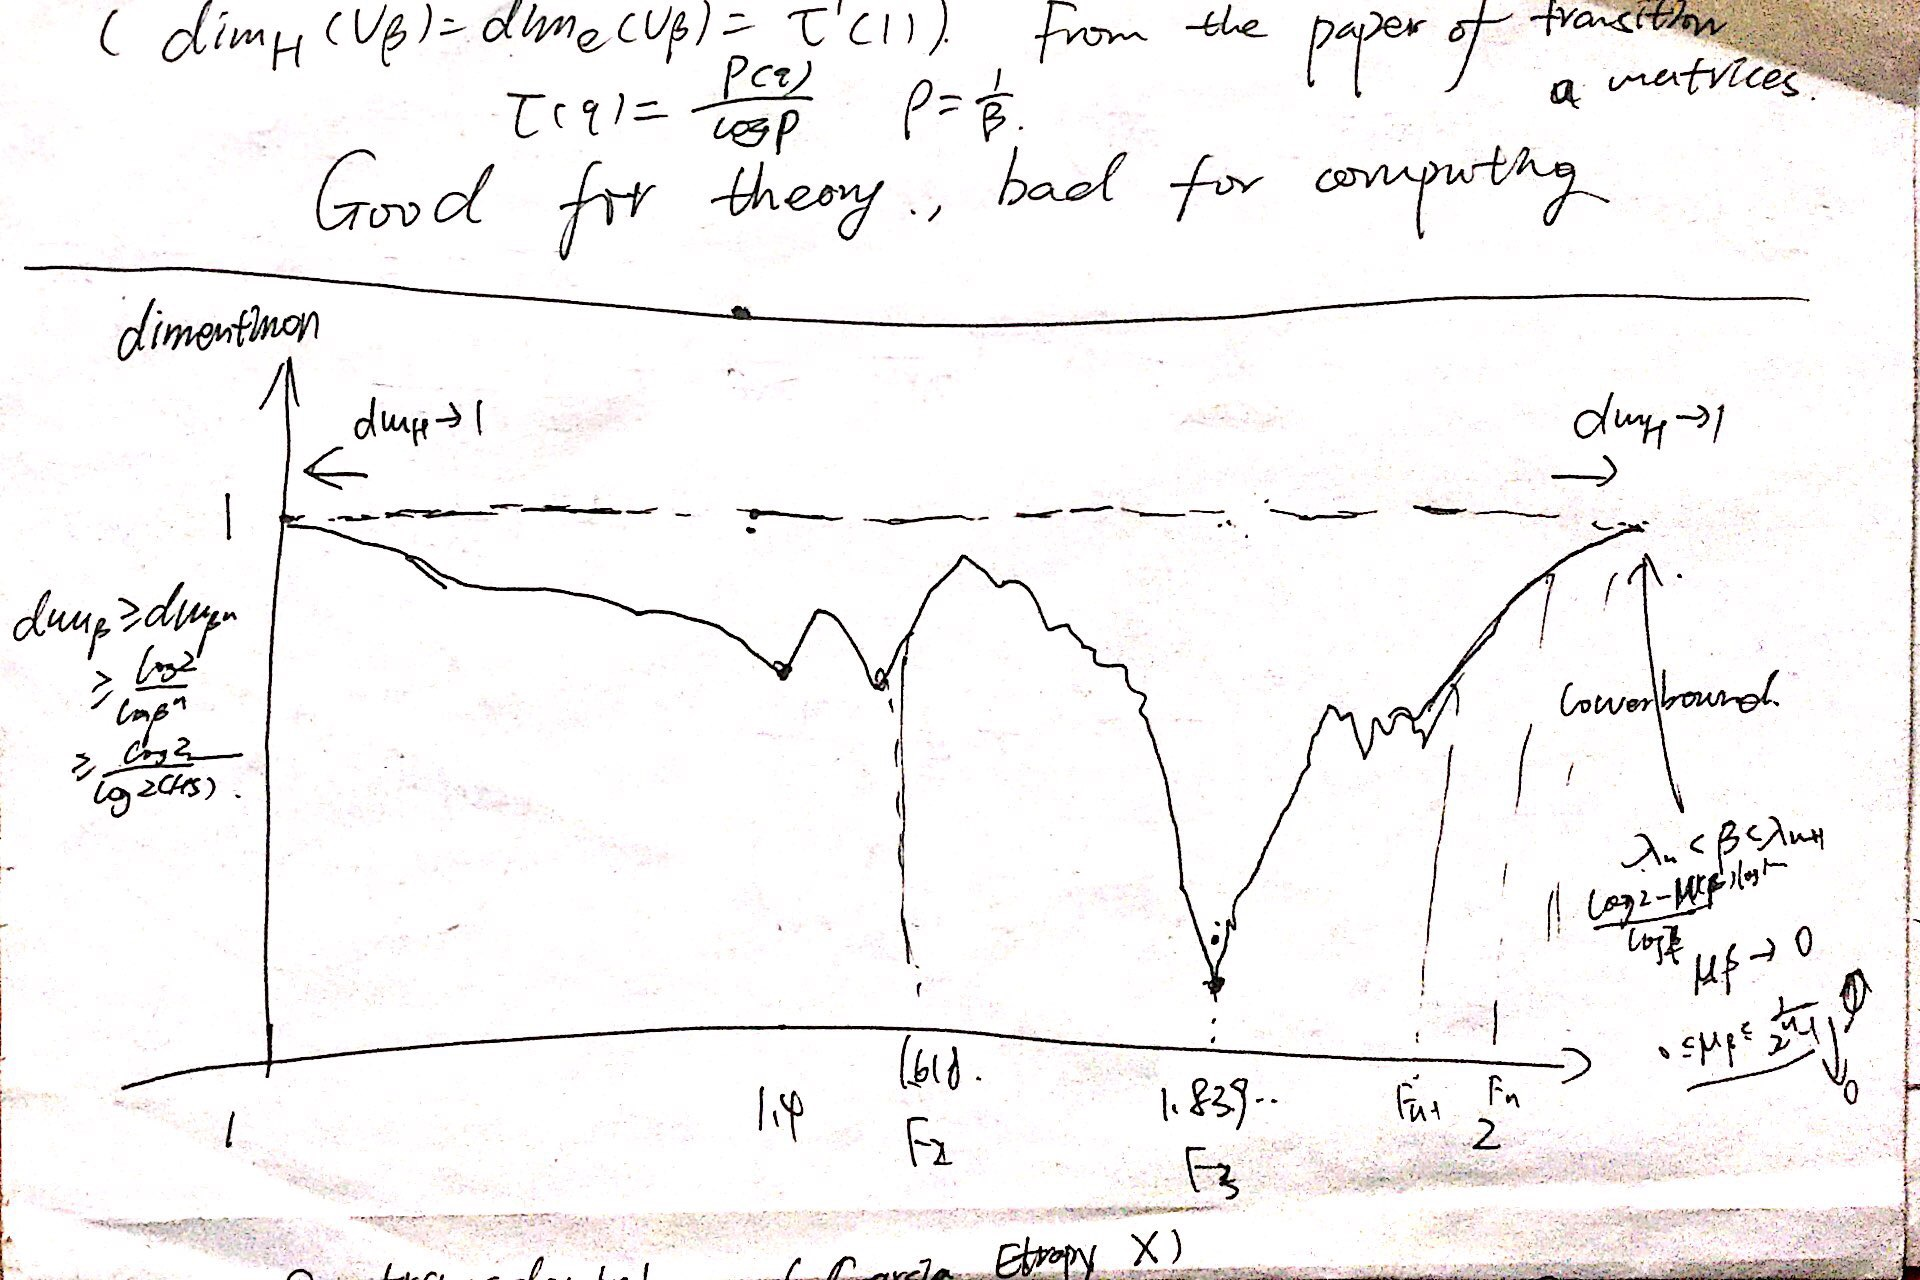
\includegraphics[width=\textwidth,height=0.65\textheight]{system2}
		\caption{Bernoulli卷积Hausdorff维数关于$ \beta $的粗略分布}
	\end{figure}
\end{frame}








%------------------------------------------------
\appendix
\begin{frame}
\frametitle{参考文献}\small
\footnotesize{
%	\bibliographystyle{plain}
%	\bibliography{openingref}
\begin{thebibliography}{99} % Beamer does not support BibTeX so references must be inserted manually as below
\bibitem[SixtyYears]{Sixtyyears}  Peres Y., Schlag W., Solomyak B. (2000) Sixty Years of Bernoulli Convolutions. In: Bandt C., Graf S., Zähle M. (eds) Fractal Geometry and Stochastics II. Progress in Probability, vol 46. Birkhäuser, Basel
\bibitem[DJFeng1]{DJFeng1} Shigeki Akiyama, De-Jun Feng, Tom Kempton, Tomas Persson; On the Hausdorff Dimension of Bernoulli Convolutions, International Mathematics Research Notices, , rny209, https://doi.org/10.1093/imrn/rny209
\bibitem[DJFeng2]{DJFeng2} FENG, DE-JUN. “SMOOTHNESS OF THE $L^{q}$-SPECTRUM OF SELF-SIMILAR MEASURES WITH OVERLAPS.” Journal of the London Mathematical Society, vol. 68, no. 1, 2003, pp. 102–118., doi:10.1112/S002461070300437X.
\bibitem[DJFeng3]{DJFeng3} De-Jun Feng, Yang Wang, 2004, 'Bernoulli convolutions associated with certain non-Pisot numbers', Advances in Mathematics, vol. 187, no. 1, pp. 173-194

\end{thebibliography}
}
\end{frame}


\begin{frame}
\frametitle{参考文献}\small
\footnotesize{
	%	\bibliographystyle{plain}
	%	\bibliography{openingref}
	\begin{thebibliography}{99} % Beamer does not support BibTeX so references must be inserted manually as below
	
		\bibitem[Niki1]{Niki1}  Kevin G. Hare \& Nikita Sidorov (2018) A Lower Bound for the Dimension of Bernoulli Convolutions, Experimental Mathematics, 27:4, 414-418, DOI: 10.1080/10586458.2017.1301841 
		\bibitem[Falconer]{Falconer} Falconer, K. J. Fractal Geometry. Wiley, 1990.
		\bibitem[Mattila]{Mattila} Mattila, Pertti. Geometry of Sets and Measures in Euclidean Spaces: Fractals and Rectifiability. Cambridge University Press, 1995.
		
	\end{thebibliography}
}
\end{frame}
%------------------------------------------------

\begin{frame}
\Huge{\centerline{谢谢!}}
\end{frame}

%----------------------------------------------------------------------------------------

\end{document}